%----------------------Pre-Amble-------------------------
\documentclass{MathNotes}
\newenvironment{example}[1]
{\begin{BlueBox}{Example}{#1}}{\end{BlueBox}}

\newenvironment{definition}[1]
{\begin{RedBox}{Definition}{#1}}{\end{RedBox}}
    
\newenvironment{note}[1]
{\begin{YellowBox}{Note}{#1}}{\end{YellowBox}}

\newenvironment{theorem}[1]
{\begin{GrayBox}{Theorem}{#1}}{\end{GrayBox}}

\newenvironment{practice}[2]
{\begin{PurpleBox}{\texorpdfstring{#1}\Big|You Try}{#2}}{\end{PurpleBox}}

\newcommand{\br}{
\begin{center}
\line(1,0){4ex}
\end{center}}
%----------------------Author Information-----------------
\title{MATH-2417.001 Notes}
\author{Minh Nguyen}

%---------------------Document Begin-----------------------
% \usepackage{layout}
\begin{document}
% \begin{center}
%     \layout*
% \end{center}
\newpage
\maketitle
\pagenumbering{roman}
\tableofcontents
\newpage
\section*{Author's Notes}
This is my very first project that I wrote in \LaTeX, but I hope you enjoy
the notes that I poured my blood, sweat, and tears into \emoji{sob} 
\br
These notes are based off of the textbook \textit{Calculus 11e} by 
\textit{Ron Larson} and \textit{Bruce Edwards}, as well as the lectures of 
professor \textit{Carlos Arreche} from the \textit{Fall 2023} semester.
\br
Practice problems are also found within the notes. The answers for the practice
problems are found at the end of the notes. Please try them yourself so that
you can get a hang of the subject!
\br
If you have any complaints, or suggestions regarding these notes, please
email me at \newline\href{mailto:minh.nguyen7@utdallas.edu}{mdn220004@utdallas.edu}
\newpage
\pagenumbering{arabic}

\section{Limits}\label{sec:1}
\subsection{Finding Limits Graphically \& Numerically}

\begin{multicols}{2}[]
\begin{theorem}{Informal Definition of Limit}
    \[\lim_{x\to c}f(x)=L\] 
    As $x$ gets closer to $c$, the value of $f(x)$ becomes $L$
\end{theorem}


Limits also depend on what direction\footnote{If the limits from the left and
right don't match, then the limit \textit{doesn't exist}} you're coming from:
\begin{tabular}{ |l|c| }
    \hline
    Meaning & Math Expression\\
    \hline
    \hline
    From the right & $\lim_{x\to c^+}f(x)$ \\
    \hline
    From the left & $\lim_{x\to c^-}f(x)$ \\
    \hline
\end{tabular}
\end{multicols}

\begin{example}{Estimating Graphically and Numerically}\label{ex:1.1}
    Consider the function $f(x)=\frac{x^3-1}{x-1}$:
    \begin{center}
        \begin{tikzpicture}
            \begin{axis}[
                    axis lines        = box,
                    xmin              = 0,
                    xmax              = 2,
                    ymin              = 0,
                    ymax              = 8,
                    xlabel            = $x$,
                    ylabel            = $f(x)$,
                    variable          = t,
                    trig format plots = rad,
                ]

                \addplot [
                    domain=0:2,
                    smooth,
                    color=blue,
                ]
                {(x^3-1)/(x-1)};
                \addlegendentry{$f(x)=\frac{x^3-1}{x-1}$}

                \addplot [
                    color=blue,
                    mark=o
                ]
                coordinates {(1,3)};
            \end{axis}
        \end{tikzpicture}

        \begin{tabular}{ |c||c|c|c|c|c|c|c| }
            \hline
            x    & 0.9 & 0.99 & 0.999 & 1 & 1.001 & 1.01 & 1.1\\
            \hline
            f(x) & 2.71 & 2.97 & 2.997 &DNE& 3.003 & 3.03 & 3.31 \\
            \hline
        \end{tabular}
    \end{center}

    Notice how in both the \textbf{table and graph}, $f(x)$ looks like it's
    approaching $f(x)=3$ when $x=1$
\end{example}

\subsubsection{When Limits Fail to Exist}
\begin{note}{Limits Don't Exist When}
    \begin{itemize}
        \item $\lim_{x\to c^-}f(x)\neq \lim_{x\to c^+}f(x)$
        \item $f(x)$ is a violently oscillating function
    \end{itemize}
\end{note}

\subsubsection{A Formal Definition}

\begin{multicols}{2}
    \begin{theorem}{Limits via. $\varepsilon - \delta$}
        The statement $\lim_{x\to c}f(x)=L$ means that for each $\varepsilon > 0$ there 
        exists $ \delta>0 $ such that if $0<\lvert x-c \rvert < \delta$ then
        $\lvert f(x)-L \rvert < \varepsilon$
    \end{theorem}

    \begin{center}
        \begin{tikzpicture}
            \begin{axis}[
                    scale only axis,
                    width  = 5cm,
                    xmin   = 0,
                    xmax   = 0.85,
                    ymin   = 0,
                    ymax   = 1,
                    xtick  = \empty,
                    ytick  = \empty,
                    xlabel = \empty,
                    ylabel = \empty,
                    clip   = false,
                    smooth,
                ]

                \addplot[
                    domain=0:0.85, 
                    samples=100, 
                    color=red,
                ]{sqrt(x)};

                % add open dot for removable discontinuity
                \addplot [
                    color=blue,
                    mark=o
                ] coordinates {(0.4225,0.65)};

                % Epsilon-delta lines
                \draw [dashed, blue] (0, 0.75) -- (0.5625, 0.75);
                \draw [dashed, blue] (0, 0.65) -- (0.4225, 0.65);
                \draw [dashed, blue] (0, 0.55) -- (0.3025, 0.55);
                \draw [dashed, blue] (0.5625, 0) -- (0.5625, 0.75);
                \draw [dashed, blue] (0.4225, 0) -- (0.4225, 0.65);
                \draw [dashed, blue] (0.3025, 0) -- (0.3025, 0.55);

                % Labels
                \node[below] at (0.5625, 0) {c + \delta};
                \node[below] at (0.4225, 0) {c};
                \node[below] at (0.3025, 0) {c - \delta};
                \node[left] at (0, 0.75) {L + \varepsilon};
                \node[left] at (0, 0.65) {L};
                \node[left] at (0, 0.55) {L - \varepsilon};
                \node[right] at (0.4225, 0.65){(c, L)};

            \end{axis}
        \end{tikzpicture}
    \end{center}
\end{multicols}
Refer back to finding limits numerically (example \ref{ex:1.1}):
\begin{itemize}
    \item $\pm\varepsilon$ would be the values on the row $f(x)$
    \item $\pm\delta$ would be the values on the row $x$
\end{itemize}


\begin{practice}{\hyperref[ans:1.1.2-1]{1}}{Proving Limits via. $\varepsilon-\delta$ Definition}
    \label{prac:1.1.2-1}
    Consider $f(x)=10x-6$, prove that $\displaystyle\lim_{x\to 3}f(x)=24$ using the 
    $\epsilon-\delta$ definition
\end{practice}

\subsection{Evaluating Limits Analytically}

\subsubsection{Properties of Limits}

\marginpar{$\mathbb{R}=$all real numbers\\$\mathbb{N}=$all natural numbers}
\begin{multicols}{2}[]
    \begin{theorem}{Basic Limit Properties}
        Let $\{b, c\}=\mathbb{R}$, $n=\mathbb{N}$:

        \begin{enumerate}
            \item $\lim_{x\to c}x=c$ 
            \item $\lim_{x\to c}b=b$ 
            \item $\lim_{x\to c}x^n=c^n$
        \end{enumerate}
    \end{theorem}

    \begin{example}{Evaluating Basic Limits}
        \begin{center}
            \begin{align*}
                \lim_{x\to 2}5&=5 \\  
                \lim_{x\to 4}x&=4 \\
                \lim_{x\to 5}x^2&=25
            \end{align*}
        \end{center}
    \end{example}
\end{multicols}

\marginpar{$f(g(x))$ may also be written as $f\circ g$ }
\begin{theorem}{Limit Properties}
    Let $\{b, c\}=\mathbb{R}$, $n=\mathbb{N}$, and $f$ and $g$ are functions
    with limits:
    \begin{displaymath}
        \lim_{x\to c}f(x)=L\hspace{2ex}\text{and}\hspace{2ex}\lim_{x\to c}g(x)=K
    \end{displaymath}

    \begin{enumerate}
        \item $\lim_{x\to c}\l[ b\cdot f(x) \r]=b\cdot L$
        \item $\lim_{x\to c}\l[ b\pm f(x) \r]=b\pm L$
        \item $\lim_{x\to c}\l[ f(x)\cdot g(x) \r]=L\cdot K$
        \item $\lim_{x\to c}\frac{f(x)}{g(x)}=\frac{L}{K}, K\neq 0$
        \item $\lim_{x\to c}\l[ f(x)\r] ^n=L^n$
        \item $\lim_{x\to c}\sqrt[n]x=\sqrt[n]{c}$
        \item $\lim_{x\to c}f\bigl(g(x)\bigr)=f\bigl(\lim_{x\to c}g(x)\bigr)=f(K)$
    \end{enumerate}
\end{theorem}

\begin{example}{Limit of Polynomial}
    \begin{align*}
        \lim_{x\to 5}\l[ 3x^3+4 \r] &= \lim_{x\to 5} 3x^3 + \lim_{x\to 5}4\\
        &= 3 \cdot \lim_{x\to 5}x^3 + \lim_{x\to 5}4\\
        &= 3 \cdot (5)^3 + 4=379
    \end{align*}
\end{example}

\begin{theorem}{Limits of Polynomial/Rationals}
    Let $c=\mathbb{R}$ and $p$ be a polynomial function:
    \begin{displaymath}
        \lim_{x\to c}p(x)=p(c)
    \end{displaymath}

    Let $r$ be a rational function $r(x)=\frac{p(x)}{q(x)}$ and $c=\mathbb{R}$
    such that $q(c)\neq 0$:

    \begin{displaymath}
        \lim_{x\to c}r(x)=r(c)=\frac{p(r)}{q(r)}
    \end{displaymath}
\end{theorem}

\newpage
\subsubsection{Squeeze Theorem}\label{sec:1.2.2}

\marginpar{
    Open/closed interval continuity will be discussed later in section
    \ref{sec:1.3.1}. 
}
\begin{multicols}{2}[]
    \begin{theorem}{The Squeeze Theorem}
        Suppose $h(x)\leq f(x) \leq g(x)$ for all $x$ in an open interval
        \textit{except} when $x=c$
        \br

        Also suppose that $\displaystyle\lim_{x\to c}h(x)=L=\lim_{x\to c}g(x)$ i.e. they share
        the same limit.
        \br

        This would mean that $\lim_{x\to c}f(x)=L$
    \end{theorem}

    \begin{theorem}{Trigonomic Limits}
        \begin{enumerate}
            \item $\displaystyle\lim_{x\to 0}\frac{\sin x}{x}$
            \item $\displaystyle\lim_{x\to 0}\frac{1 - \cos x}{x} = 1$
        \end{enumerate}
    \end{theorem}

    \begin{center}
        \begin{tikzpicture}
            \begin{axis}[
                    axis lines        = box,
                    xmin              = -5,
                    xmax              = 5,
                    ymin              = -5,
                    ymax              = 5,
                    xtick             = \empty,
                    ytick             = \empty,
                    xlabel            = \empty,
                    ylabel            = \empty,
                    trig format plots = rad,
                    width             = 15em,
                    title             = {Squeeze Theorem}
                ]

                \addplot [
                    smooth,
                    color=red,
                ]{x^2};
                \addplot [
                    smooth,
                    color=green,
                ]{-x^2};

                % add shading to regions

                \addplot [
                    draw=none,
                    pattern = north west lines,
                    pattern color=red,
                    smooth,
                ]{x^2};
                \addplot [
                    smooth,
                    draw=none,
                    pattern = north west lines,
                    pattern color=green,
                ]{-x^2};


                \addplot [
                    smooth,
                    color=blue,
                ]{x * sin(x)};

                \addplot [
                    color=black,
                    mark=*,
                ]coordinates{(0, 0)};

                \node[right] at (0, 0) {(c, L)};
            \end{axis}
        \end{tikzpicture}
    \end{center}
\end{multicols}

\begin{practice}{\hyperref[ans:1.2.2-1]{1}}{Squeeze Theorem}\label{prac:1.2.2-1}
    Show that
    $\displaystyle\lim_{x\to 0}(\cos(\frac{2\pi}{3x})\cdot\sqrt{x^3+x^2})=0$
    using the Squeeze Theorem
\end{practice}
\begin{practice}{\hyperref[ans:1.2.2-2]{2}}{Trigonomic Limit}\label{prac:1.2.2-1}
    Evaluate:
    $$\lim_{x\to 0}\frac{\tan(3x)}{4x+\sin(2x)}$$
    \textbf{Hint:} Break it down to the trigonomic functions you know
    how to take a limit of!
\end{practice}

\subsection{Continuity}

\begin{multicols}{2}
\begin{definition}{Definition of Continuity}
    A function $f$ is continuous if:
    \begin{enumerate}
        \item $f(c)$ exists
        \item $\lim_{x\to c}f(x)$ exists
        \item $f(c)=\lim_{x\to c}f(c)$
    \end{enumerate}
\end{definition}

\begin{practice}{\hyperref[ans:1.3-1]{1}}{Determine Continuity}\label{prac:1.3-1}
    Determine if the function is continuous at $x=2$
\end{practice}
\end{multicols}

\begin{note}{Continuous Functions}
    The following functions are always continuous \textit{everywhere
    they're defined}:
    \begin{itemize}
        \item polynomial functions
        \item rational functions
        \item radical functions
        \item trigonomic functions
    \end{itemize}
\end{note}

\subsubsection{Open and Closed Intervals}\label{sec:1.3.1}
A function is continuous on an \textbf{open interval} $(a, b)$ if
$f(x)=c$ for each $c$ in $(a, b)$

A function is continuous on a \textbf{closed interval} $[a, b]$ if:
\begin{itemize}
    \item $f(x)$ is continuous on $(a, b)$
    \item $\lim_{x\to b^-}f(x)=f(b)$
    \item $\lim_{x\to a^+}f(x)=f(a)$
\end{itemize}

\begin{theorem}{Intermediate Value Theorem}
    If $f(x)$ is continuous on $[a, b], a\neq b$, and $k$ is any number
    between $f(a)$ and $f(b)$, then there exists a number $c$ in
    $[a, b]$ such that: $$f(c)=k$$
\end{theorem}

\begin{practice}{\hyperref[ans:1.3.1-1]{1}}{Intermediate Value Thorem}
    \label{prac:1.3.1-1}
    Use the Intermediate Value Theorem to prove that $x^3+x^2=1$ has at least
    one solution on the interval $(-1, 2)$
\end{practice}

\subsubsection{Discontinuities}

\begin{multicols}{2}[
        There are two cases where discontinuities happen: \marginpar{Another
        example of removable discontinuity is in example \ref{ex:1.1}}
    ]{
        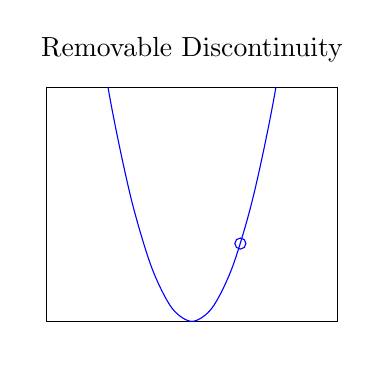
\begin{tikzpicture}
            \begin{axis}[
                    axis lines        = box,
                    xmin              = -3,
                    xmax              = 3,
                    ymin              = 0,
                    ymax              = 3,
                    xtick             = \empty,
                    ytick             = \empty,
                    xlabel            = \empty,
                    ylabel            = \empty,
                    trig format plots = rad,
                    width             = 15em,
                    title             = {Removable Discontinuity}
                ]

                \addplot [
                    smooth,
                    color=blue,
                ]{x^2};

                \addplot [
                    color=blue,
                    mark=o
                ]coordinates {(1,1)};
            \end{axis}
        \end{tikzpicture}
        \\
        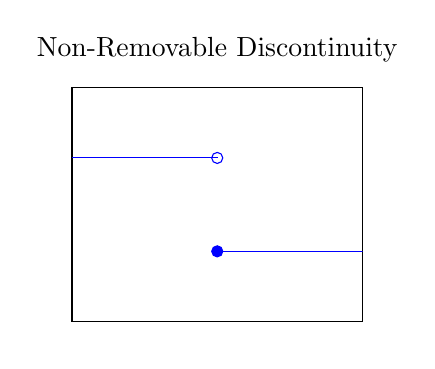
\begin{tikzpicture}
            \begin{axis}[
                    axis lines        = box,
                    xmin              = -5,
                    xmax              = 5,
                    ymin              = -5,
                    ymax              = 5,
                    xtick             = \empty,
                    ytick             = \empty,
                    xlabel            = \empty,
                    ylabel            = \empty,
                    trig format plots = rad,
                    width             = 15em,
                    title             = {Non-Removable Discontinuity}
                ]

                \addplot [
                    smooth,
                    color=blue,
                    domain=-5:0
                ]{2};

                \addplot [
                    smooth,
                    color=blue,
                    domain=0:5
                ]{-2};

                \addplot [
                    color=blue,
                    mark=o
                ]coordinates {(0,2)};

                \addplot [
                    color=blue,
                    mark=*
                ]coordinates {(0,-2)};

            \end{axis}
        \end{tikzpicture}
    }
\end{multicols}

\subsubsection{Asymptotes}
\begin{multicols}{2}[
\begin{definition}{Asymptotes}
    \begin{multicols}{2}{
            Vertical asymptote are when:
            \begin{displaymath}
                \lim_{x\to c^\pm}f(x)=\pm\infty
            \end{displaymath}
            \\
        }
        {
            Horizontal asymptote is:
            \begin{displaymath}
                \lim_{x\to \pm\infty}f(x)=L
            \end{displaymath}
        }
    \end{multicols}
\end{definition}
]{
\begin{center}
        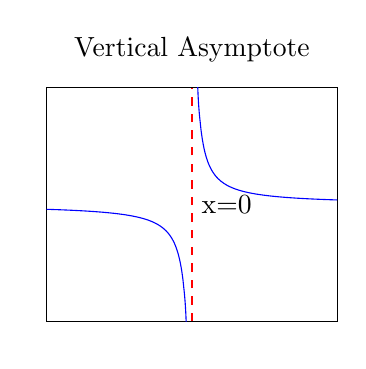
\begin{tikzpicture}
            \begin{axis}[
                    axis lines        = box,
                    xmin              = -5,
                    xmax              = 5,
                    ymin              = -5,
                    ymax              = 5,
                    xtick             = \empty,
                    ytick             = \empty,
                    xlabel            = \empty,
                    ylabel            = \empty,
                    trig format plots = rad,
                    width             = 15em,
                    title             = {Vertical Asymptote}
                ]

                % it draws a vertical line if i don't do this
                \addplot [
                    smooth,
                    color=blue,
                    samples=50,
                    domain=-5:-.1
                ]{1/x};
                \addplot [
                    smooth,
                    color=blue,
                    samples=50,
                    domain=.1:5
                ]{1/x};

                \draw [dashed, red] (0, -5) -- (0, 5);
                \node [right] at (0, 0) {x=0};

            \end{axis}
        \end{tikzpicture}
        $f(x)=\frac{1}{x}$
\end{center}
}
{
\begin{center}
        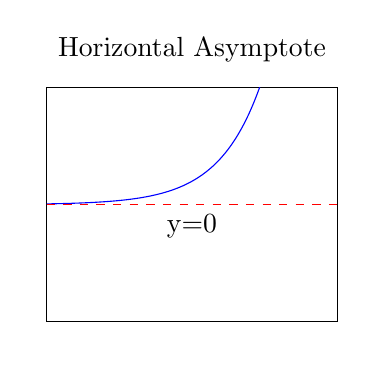
\begin{tikzpicture}
            \begin{axis}[
                    axis lines        = box,
                    xmin              = -5,
                    xmax              = 5,
                    ymin              = -5,
                    ymax              = 5,
                    xtick             = \empty,
                    ytick             = \empty,
                    xlabel            = \empty,
                    ylabel            = \empty,
                    trig format plots = rad,
                    width             = 15em,
                    title             = {Horizontal Asymptote}
                ]

                % it draws a vertical line if i don't do this
                \addplot [
                    smooth,
                    color=blue,
                    samples=50,
                ]{2^x};

                \draw [dashed, red] (-5, 0) -- (5, 0);
                \node [below] at (0, 0) {y=0};

            \end{axis}
        \end{tikzpicture}
        $f(x)=2^x$
\end{center}
}
\end{multicols}

\begin{note}{}
    We can infer something from vertical asymptotes from this graph:
    As the denominator becomes closer to zero, and it's a positive number, then
    the $f(x)$ will approach $\infty$. If the denominator approaches zero and
    is negative, then $f(x)$ will approach $-\infty$
\end{note}

\begin{multicols}{2}
\begin{practice}{\hyperref[ans:1.3.3-1]{1}}{Curveball Asymptote}\label{prac:1.3.3-1}
    Find the asymptotes:
    \begin{displaymath}
        f(x)=\frac{\sqrt{(x-1)(x-3)}}{(x-2)(x-4)}
    \end{displaymath}
\end{practice}

\begin{practice}{\hyperref[ans:1.3.3-2]{2}}{Curveball Trigonometry}\label{prac:1.3.3-2}
    Find the asymptotes:
    \begin{displaymath}
        f(x)=\frac{\sin(x)}{x^3-x}
    \end{displaymath}
\end{practice}
\end{multicols}

\newpage
\section{Differentiation}
Derivatives are essentially the \textit{slope} of the function at a
certain point

They also \textit{cannot exist} where the limit doesn't exist at the 
function

\marginpar{This comes in handy when solving physics problems!}
\begin{note}{Derivatives and Rate of Change}
To elaborate more on this, the derivative of a function $f(x)$ at point $x=c$
is the instantaneous rate of change: $$f'(x)\Big|_{x=c}$$ The average rate of
change of the function on the interval $[a, b]$ is written as such:
$$\frac{f(b)-f(a)}{b-a}$$
\end{note}

\subsection{Derivatives and Tangent Lines}
%graph some examples of tanget line
Some mathematicians were trying to find out how to draw a line that intersects 
a function at \textit{only one point}:

\begin{center}
        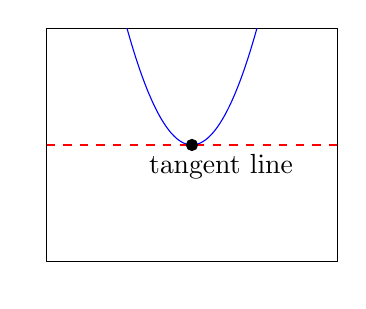
\begin{tikzpicture}
            \begin{axis}[
                    axis lines        = box,
                    xmin              = -5,
                    xmax              = 5,
                    ymin              = -5,
                    ymax              = 5,
                    xtick             = \empty,
                    ytick             = \empty,
                    xlabel            = \empty,
                    ylabel            = \empty,
                    trig format plots = rad,
                    width             = 15em,
                ]

                % it draws a vertical line if i don't do this
                \addplot [
                    smooth,
                    color=blue,
                    samples=50,
                ]{x^2};

                \addplot [
                    color=black,
                    mark=*
                ]coordinates{(0, 0)};

                \draw [dashed, red] (-5, 0) -- (5, 0);

                \node[below] at (1, 0) {tangent line};
            \end{axis}
        \end{tikzpicture}
\end{center}

However, it takes \textit{two points} to draw a line, so they were confuzzled.

You can just Google up the rest of the lore behind the definition of a limit, 
but it boils down to this:
\begin{theorem}{Derivative via. Limits}
    \begin{displaymath}
        \lim_{h\to 0}\frac{f(x+h)-f(x)}{h}=f'(c)\text{ and }
        \lim_{x\to a}\frac{f(x)-f(a)}{x-a}=f'(c)
    \end{displaymath}
\end{theorem}

\begin{note}{Alternative Ways of Writing a Derivative}
There are other ways that mathematicians defined derivative:
\begin{multicols}{2}[]
    \begin{itemize}
        \item $f'(x)$
        \item $\frac{dy}{dx}$
        \item $\frac{d}{dx}f(x)$
        \item $Dx(y)$
    \end{itemize}
\end{multicols}
This isn't essential to know, but it's pretty useful to see how other
mathematicians may express derivatives
\end{note}

\begin{theorem}{Continuity of Derivatives}
    If function $f(x)$ is differentiable at $x=c$, then it is 
    \textit{also continuous} at $x=c$
\end{theorem}

\begin{practice}{\hyperref[ans:2.1-1]{1}}{Finding the Tangent Line}\label{prac:2.1-1}
    Find the tangent lines to $f(x)=x^2+1$ at $(-2, 5)$
\end{practice}

\subsection{Rules of Derivatives}
Finding derivatives with the limit definition can get pretty exhausting, so
mathematicians came up with a lot of shortcuts to evaluate derivatives much
quicker. This is a pretty lengthy section, because of the many practice example 
problems I'll be putting in this section, but here are the rules in short:

\begin{theorem}{Derivative Rules}
    \begin{align*}
        \text{Let: } f(x)&= \text{a function}\\
                     g(x)&= \text{another function}\\
                       c &= \text{a constant}
    \end{align*}
    \begin{tabular}{ cll }
        1. & Constant & $\frac{d}{dx}c=0$\\
        2. & Power & $\frac{d}{dx}x^n=nx^{n-1}$\\
        3. & Sum and Difference & $\frac{d}{dx}[f(x)\pm g(x)]=f'(x)\pm g'(x)$\\
        4. & Product& 
            $\frac{d}{dx}[f(x)g(x)]=f(x)g'(x)+g(x)f'(x)$\\
        5. & Quotient& 
            $\frac{d}{dx}[\frac{f(x)}{g(x)}]=
             \frac{g(x)\cdot f'(x)-f(x)\cdot g'(x)}{\bigl(g(x)\bigr)^2}$\\
        6. & Trigonometry& $\frac{d}{dx}\sin(x)=\cos(x)$\\
        && $\frac{d}{dx}\cos(x)=-\sin(x)$\\
        && $\frac{d}{dx}\tan(x)=\sec^2(x)$\\
        && $\frac{d}{dx}\cot(x)=-\csc^2(x)$\\
        && $\frac{d}{dx}\sec(x)=\sec(x)\tan(x)$\\
        && $\frac{d}{dx}\csc(x)=-\csc(x)\cot(x)$\\
        7. & Chain & $\frac{d}{dx}f(g(x))=g'(x)\cdot f'(g(x))$\\
    \end{tabular}
\end{theorem}

\marginpar{You don't have to simplify completely on open-ended questions!}
\begin{example}{Power Rule}
    \begin{multicols}{2}
        \begin{enumerate}
            \item $\displaystyle\frac{d}{dx}(3x^2+4x)=6x+4$
            \item $\displaystyle\frac{d}{dx}\sqrt{x}=\frac{d}{dx}x^{\frac{1}{2}}
                =\frac{1}{2}x^{-\frac{1}{2}}$
            \item $\displaystyle\frac{d}{dx}\sqrt[3]{x^2}=\frac{d}{dx}x^{\frac{2}{3}}
                =x^{-\frac{1}{3}}$
        \end{enumerate}
    \end{multicols}
\end{example}

\begin{example}{Product and Quotient Rule}
    \begin{enumerate}
        \item $\displaystyle\frac{d}{dx}(2x+3)(3x^2+1)=(2x+3)(6x)+(3x^2+1)(2)$
        \item $\displaystyle\frac{d}{dx}\frac{x^2+3}{2x-1}
            =\frac{(2x-1)(2x)-(x^2+3)(2)}{(2x-1)^2}$
    \end{enumerate}
\end{example}

\newpage
\marginpar{$u$-substitution is a good method for solving chain rule problems:}
\begin{example}{Chain Rule}
    $$
    \frac{d}{dx}\sin(x^2+1) \\
    $$
    \begin{align*}
        u&=x^2+1,&v&=\sin(u)\\
        u'&=2x,&v'&=\cos(u)\\
        &&v'&=\cos(x^2+1)\\
    \end{align*}
    \begin{align*}
        &=u'\cdot v'\\
        &=2x\cdot\cos(x^2+1)
    \end{align*}
\end{example}
\marginpar{Remember: $\sin^2(\theta)+\cos^2(\theta)=1$}
\begin{example}{$\sin$ and $\cos$ Rule}
    \begin{enumerate}
        \item $\displaystyle\frac{d}{dx}
            \bigl(2\sin(\theta)+3\cos(\theta)-\frac{4}{\theta}\bigr)=
            2\cos(\theta)-3\sin(\theta)+\frac{4}{\theta^2}
            $
        \item $\displaystyle\frac{d}{dx}\bigl(x^2+2\cos(x)\bigr)=2x-2\sin(x)$
        \item $\displaystyle\frac{d}{d\theta}\bigl(\tan(\theta)\bigr)
            =\frac{d}{d\theta}\bigl(\frac{\sin(\theta)}{\cos(\theta)}\bigr)
            =\frac{\cos^2(\theta)+\sin^2(\theta)}{\cos^2(\theta)}
            =\sec^2(\theta)$
    \end{enumerate}
\end{example}

\begin{multicols}{2}
    \begin{practice}{\hyperref[ans:2.2-1]{1}}{Find Horizontal Tangents}
        \label{prac:2.2-1}
        Find the horizontal tangents of $f(x)=x^4-2x^2+3$
    \end{practice}
    \begin{practice}{\hyperref[ans:2.2-2]{2}}{Find the Derivative}
        \label{prac:2.2-2}
        Find the derivative of \newline$\displaystyle f(x)=\big((x^2+3)^5+x\big)^2$
    \end{practice}
\end{multicols}

\newpage
\subsection{Higher Order Derivatives}
You can take a derivative of derivative:
\begin{displaymath}
    \frac{d}{dx}\big[\frac{d}{dx}f(x)\big]=\frac{d^2}{dx^2}\big[f(x)\big]
    =f''(x)
\end{displaymath}
\begin{example}{Finding the Second Derivative}
    Finding $f''(x)$ when $f(x)=\frac{2x}{x+1}$:
    \begin{align*}
        f'(x)&=\frac{2\cdot(x+1)-(2x)\cdot 1}{(x+1)^2}\\
        &=\frac{2}{(x+1)^2}\\
        \\
        f''(x)&=-\frac{4(x+1)}{(x+4)^4}
    \end{align*}
\end{example}
You can do this for however many times you want to!
\begin{practice}{\hyperref[ans:2.3.1-1]{2.3.1-1}}{Velocity and Acceleration}
    \label{prac:2.3.1-1}
    A ball is thrown up into the air, and its position can be modeled into
    of feet as a function of time: $f(t)=-5(t-2)^2+20$. Find the acceleration
    of the ball just as it's about to hit the ground again.
\end{practice}
\begin{note}{Taking Beyond the Third Derivative}
    Taking $f'''(x)$ and beyond, it'll start to be tedious writing all of those
    apostrophes. Mathematicians often write it like this:
    $$\frac{d^n}{dx^n}\big[f(x)\big]=f^{(n)}(x)$$
\end{note}

\subsection{Implicit Differentiation}
So far, we've been using \textit{explicit differentiation}, which is when $y$
can be isolated on one side of the equation where $y$ is a function of $x$.

What if that's not possible?

That's where \textit{implicit differentiation comes through}. Here are the 
steps on how to do that:

\begin{note}{Steps for Implicit Differentiation}
    \begin{enumerate}
        \item For all terms of $x$ and $y$, derive in respect to $x$:
            ($\frac{d}{dx}$) 
        \item Isolate all terms with $\frac{dy}{dx}$
        \item Factor out $\frac{dy}{dx}$ where the terms with $\frac{dy}{dx}$
            are isolated
        \item Solve for $\frac{dy}{dx}$
    \end{enumerate}
\end{note}
It's also important to understand that derivative rules don't have to just
apply to terms of $x$. The example on the next page shows an implicit
differentiation using the product rule on \textit{x and y}:
\begin{example}{Implicit Differentiation with Product Rule}
    Let's follow those steps to find the derivative of $$x^2y+y^2x=-2$$

    Begin by deriving all terms in respect to $x$:
    \begin{align*}
        x^2y+y^2x&=-2\\
        \frac{d}{dx}x^2y+\frac{d}{dx}y^2x&=\frac{d}{dx}-2\\
        (x^2\cdot 1\frac{dy}{dx}+y\cdot2x\frac{dx}{dx})
            +(y^2\cdot1\frac{dx}{dx}+x\cdot2y\frac{dy}{dx})&=0\\
        x^2\frac{dy}{dx}+2xy+y^2+2yx\frac{dy}{dx}&=0\\
    \end{align*}
    Next, isolate terms with $\frac{dy}{dx}$:
    $$x^2\frac{dy}{dx}+2yx\frac{dy}{dx}=-2xy-y^2$$
    Factor out $\frac{dy}{dx}$
    $$(x^2+2yx)\frac{dy}{dx}=-2xy-y^2$$
    Solve for $\frac{dy}{dx}$
    $$\frac{dy}{dx}=\frac{-2xy-y^2}{x^2+2yx}$$
\end{example}

\newpage
\begin{multicols}{2}
    \begin{practice}{\hyperref[ans:2.4-1]{2.4-1}}{Tangent Lines and Circles}
        \label{prac:2.4-1}
        Find the tangent line at $(4,-3)$ of \textit{the circle}:
        $$x^2+y^2=5^2$$
    \end{practice}
    \begin{practice}{\hyperref[ans:2.4-2]{2.4-2}}{Differentiate}\label{prac:2.4-2}
        Find the derivative of this function: $$(4x+4y)^3=64x^3+64y^3$$
    \end{practice}
\end{multicols}

\subsection{Related Rates}
Solving related-rate problems are similar to solving implicit differentiation.
However, in this case, related-rate problems are typically differentiated in
\textit{respect to time}. Additionally, related-rate problems provide given
quantities as well as quantities to find:

\begin{note}{Guideline for Related-Rate Problems}
    \begin{enumerate}
        \item Take note of all quantities \textit{given} and quantities
            \textit{yet to find} within the problem. Create a sketch if it
            helps to visualize the problem.
        \item Write equation with those quantities and rates that were
            identified in the first step.
        \item Implicitly differentiate the equation \textit{with respect to
            time}
        \item Substitute the given values, and solve for the required rate of
            change
    \end{enumerate}
\end{note}

On the next page, Let's see how those steps can be used on an example problem:
\begin{example}{Related Rate with Cylindrical Glass}
    The radius $r$ of a circle is increasing at a rate of 8 centimeters per
    minute. Find the rate of change of the area when $r = 45$ centimeters.

    The first step is to make a table of all given values and values to find:
    \begin{center}
        \begin{tabular}{l|l}
            Quantity & Value\\
            \hline
            ($r$) radius & 45 cm\\
            $\frac{dr}{dt}$ & $8\frac{cm}{min}$\\
            $\frac{dA}{dt}$ & ?\\
        \end{tabular}
    \end{center}

    The next step is to write an equation with those given quantities: For this
    case, it'll be the equation of the area of a circle: $$A=\pi r^2$$
   
    The next step is to derivatize all terms in respect to time:

    \begin{align*}
        \frac{d}{dt}(A)&=\frac{d}{dt}(\pi r^2)\\
        \frac{dA}{dt}&=2\pi r\frac{dr}{dt}
    \end{align*}

    Finally, substitute in the given values and solve for the required rate
    of change:

    \begin{align*}
        \frac{dA}{dt}&=2\pi (45cm)(8\frac{cm}{min})\\
        \frac{dA}{dt}&=720\pi\frac{cm^2}{min}
    \end{align*}

    The rate of change of the volume of the barrel is $720\pi\frac{cm^2}{min}$.
\end{example}

\begin{practice}{\hyperref[ans:2.5-1]{2.5-1}}{Triangles Galore}
    \label{prac:2.5-1}
    A ladder 25 feet long is leaning against the wall of a house. The base
    of the ladder is pulled away from the wall at a rate of 2 feet per
    second. Find the rate at which the area of the triangle is changing
    when the base of the ladder is 7 feet from the wall.
\end{practice}

\section{Applications of Differentiation}
\subsection{Extrema on an Interval}
\subsection{Rolle's Theorem \& Mean Value Theorem}
\subsection{Increasing \& Decreasing Functions---First Derivative Test}
\subsection{Concavity---Second Derivative Test}
\subsection{Limits at Infinity}
\subsection{Curve Sketching}
\subsection{Optimization Problems}
\subsection{Newton's Method}
\subsection{Differentials}


\newpage
\section{Practice Problem Answers}

\subsection*{\ref{prac:1.1.2-1}---Proving Limits via. $\varepsilon-\delta$ Definition}
\label{ans:1.1.2-1}
Consider $f(x)=10x-6$, prove that $\displaystyle\lim_{x\to 3}f(x)=24$ using the 
$\epsilon-\delta$ definition:
\br
The first thing we would have to do is to find $\delta$:
\begin{align*}
    \lvert (10x-6)-(24) \rvert &<\varepsilon  \\
    \lvert 10x-30 \rvert &<\varepsilon \\
    10\lvert x-3 \rvert &<\varepsilon \\
    \lvert x-3 \rvert &<\frac{\varepsilon}{10}
\end{align*}
\begin{align*}
    0 < \lvert x - (3)\rvert &< \delta
\end{align*}

Notice how $\delta=\frac{\epsilon}{10}$. This guarantees that
$\lvert f(x)-L \rvert < \epsilon$ whenever $0<\lvert x-c \rvert<\delta$

\subsection*{\ref{prac:1.2.2-1}---Squeeze Theorem}\label{ans:1.2.2-1}
Show that
$\displaystyle\lim_{x\to 0}(\cos(\frac{2\pi}{3x})\cdot\sqrt{x^3+x^2})=0$
using the Squeeze Theorem
\br
We know that $\displaystyle-1\leq\cos(\frac{2\pi}{3x})\leq 1$:
\begin{align*}
    -\sqrt{x^3+x^2}&\leq\cos(\frac{2\pi}{3x})\sqrt{x^3+x^2}&\leq
    \sqrt{x^3+x^2}
    \\
    \lim_{x\to 0}-\sqrt{x^3+x^2}&\leq\lim_{x\to 0}\cos(\frac{2\pi}{3x})
    \sqrt{x^3+x^2}&\leq\lim_{x\to 0}\sqrt{x^3+x^2}
    \\
    -\sqrt{(0)^3+(0)^2}&\leq\lim_{x\to 0}\cos(\frac{2\pi}{3x})
    \sqrt{x^3+x^2}&\leq\sqrt{(0)^3+(0)^2}
    \\
    0&\leq\lim_{x\to 0}\cos(\frac{2\pi}{3x})&\leq0 
\end{align*}

Because of the Squeeze Theorem, $\displaystyle\lim_{x\to 0}\cos(\frac{2\pi}{3x})=0$

\subsection*{\ref{prac:1.2.2-1}---Trigonomic Limit}\label{ans:1.2.2-2}
Evaluate:
$$\lim_{x\to 0}\frac{\tan(3x)}{4x+\sin(2x)}$$
\br

Let's start by breaking down $\tan$ into $\sin$ and $\cos$:
\begin{align*}
    \lim_{x\to 0}\frac{\tan(3x)}{4x+\sin(2x)}
    &=\lim_{x\to 0}\frac{\sin(3x)}{\cos(3x)\cdot(4x+\sin(2x))}\\
    &=\lim_{x\to 0}\frac{\sin(3x)}{4x\cos(3x)+\sin(2x)\cos(3x)}
\end{align*}
Note that we can further break down $\cos(3x)$ into $\cos(2x+x)$, which can 
be converted to the trigonomic identity:$\cos(2x)\cos(x)-\sin(2x)\sin(x)$

\begin{align*}
    &=\lim_{x\to 0}\frac{\sin(3x)}{4x\big(\cos(2x)\cos(x)-\sin(2x)\sin(x)\big)+\sin(2x)\cos(3x)}\\
    &=\lim_{x\to 0}\frac{\sin(3x)}{4x\cos(2x)\cos(x)-4x\sin(2x)\sin(x)+\sin(2x)\cos(3x)}
\end{align*}

Next, you multiply by a \textit{big 1}. In this case it would be
$\displaystyle\frac{\frac{1}{x}}{\frac{1}{x}}$:

\begin{align*}
    &=\lim_{x\to 0}\frac{\sin(3x)}{4x\cos(2x)\cos(x)-4x\sin(2x)\sin(x)+\sin(2x)\cos(3x)}\\
    &=\lim_{x\to 0}\frac{\frac{\sin(3x)}{x}}{\frac{4x\cos(2x)\cos(x)}{x}-\frac{4x\sin(2x)\sin(x)}{x}+\frac{\sin(2x)\cos(3x)}{x}}\\
    &=\lim_{x\to 0}\frac{\frac{\sin(3x)}{x}}{4\cos(2x)\cos(x)-4\sin(2x)\sin(x)+\cos(3x)\cdot\frac{\sin(2x)}{x}}\\
    &=\frac{\lim_{x\to 0}\frac{\sin(3x)}{x}}{\lim_{x\to 0}4\cos(2x)\cos(x)-\lim_{x\to 0}4\sin(2x)\sin(x)+\lim_{x\to 0}\cos(3x)\frac{\sin(2x)}{x}}\\
    &=\frac{(3)}{4\cos\big(2(0)\big)\cos\big((0)\big)-4\sin\big(2(0)\big)\sin\big((0)\big)+\cos\big(3(0)\big)(2)}\\
    &=\frac{3}{4(1)(1)-4(0)(0)+(1)\cdot 2}\\
    &=\frac{3}{4+2}=\frac{3}{6}\\
    &=\frac{1}{2}
\end{align*}

That problem was quite lengthy, but we did it \emoji{smiling-face-with-hearts}

\newpage
\subsection*{\ref{prac:1.3-1}---Determine Continuity}\label{ans:1.3-1}
Determine if the function is continuous at $x=2$

\begin{displaymath}
    f(x) = \begin{cases}
        \frac{x^2-x-2}{x-2} &\text{for } x\neq 2\\
        1 &\text{for } x=2
    \end{cases}
\end{displaymath}
\br

Let's start by plugging in $x=2$ for the case that $x\neq2$ to see if it equals
the case where $x=2$:
\begin{displaymath}
    \frac{x^2-x-2}{x-2}=\frac{(2)^2-(2)-2}{(2)-2}=\frac{0}{0}
\end{displaymath}

That's so \textit{uncool}. Let's factor it out and try again!
\begin{align*}
    \frac{x^2-x-2}{x-2} = \frac{(x-2)(x+1)}{x-2} &= x+1\\
    &=(2)+1\\
    &=3
\end{align*}

Now, we compare both that with the case where $x=2$ to see if they
are the same: $3\neq2$

\marginpar{$\therefore$ means "therefore"}
$\therefore f(x)$ is \textit{not continuous} at $x=2$!

\subsection*{\ref{prac:1.3.1-1}---Intermediate Value Theorem}\label{ans:1.3.1-1}
Use the Intermediate Value Theorem to prove that $x^3+x^2=1$ has at least
one solution on the interval $(-1, 2)$
\br
Let's treat $x^3+x^2$ as a function $f(x)$. We know that the function is 
continuous on the interval $[-1, 2]$. The next thing we have to do is to 
evaluate $f(-1)$ and $f(2)$ to compare if they are equal:
\begin{align*}
    f(-1)&=(-1)^3+(-1)^2\\
    f(2)&=(2)^3+(2)^2\\
    f(-1)&\neq f(2)\\
\end{align*}

Now that we know that $f(-1)$ and $f(2)$ are not equal, and $f(-1)<1<f(2)$, we
can conclude that there is a number '$c$' in the interval $(-1, 2)$ such that 
$f(c)=1$

\subsection*{\ref{prac:1.3.3-1}---Curveball Asymptote}\label{ans:1.3.3-1}
Find the asymptotes:
\begin{displaymath}
    f(x)=\frac{\sqrt{(x-1)(x-3)}}{(x-2)(x-4)}
\end{displaymath}
\br
You'd \textit{think} that the asymptotes are $x=\{2, 4\}$, but you must
consider the \textit{domain} at which $f(x)$ exists.
\\
Because this is a square root function, $(x-1)(x-3)$ \textit{cannot be a 
negative number}. Plugging in $x=2$ would result in a negative square root.

\subsection*{\ref{prac:1.3.3-2}---Curveball Trigonometry}\label{ans:1.3.3-2}
Find the asymptotes:
\begin{displaymath}
    f(x)=\frac{\sin(x)}{x^3-x}
\end{displaymath}
\br
Let's start by factoring out the denominator:
\begin{displaymath}
    f(x)=\frac{\sin(x)}{x(x-1)(x+1)}
\end{displaymath}
\marginpar{Moral of the story: double-check your answers!}
You'd \textit{think} that the asymptotes are $x=\{-1, 0, 1\}$. However,
$\lim_{x\to 0}f(x)=1$ --- $f(x)$ can also be re-written as this:
$\lim_{x\to 0}[\frac{\sin x}{x}] \cdot \lim_{x\to 0}[\frac{1}{(x-1)^2}]=-1$

\subsection*{\ref{prac:2.1-1}---Finding the Tangent Line}\label{ans:2.1-1}
Find the tangent lines to $f(x)=x^2+1$ at $(-2, 5)$:
\br
Let's start by finding the derivative of the function at $x=-2$:
\begin{align*}
    f'(-2)&=\lim_{h\to 0}\frac{f(-2+h)-f(-2)}{h} \\
    &=\lim_{h\to 0}\frac{\bigl((-2+h)^2+1\bigr)-(5)}{h} \\
    &=\lim_{h\to 0}\frac{h^2-4h}{h} \\
    &=\lim_{h\to 0}-4+h = -4 + (0)\\
    &=-4\\
\end{align*}
Now we must write a point-slope equation with that derivative. 
\begin{align*}
    y-y_1&=m(x-x_1) \\
    y-(5)&=(-4)(x-(-2)) \\
    y-5&=-4(x+2)
\end{align*}

Tangent line to $f(x)=x^2+1$ at $(-2, 5)$ has equation: $$y-5=-4(x+2)$$

\begin{note}{Alternative Route}
    Another way to solve this would be to find the limit of $f(x)$ when $x=c$ 
    and then plugging in $c$ with any number that you want:
    \begin{align*}
        f'(c)&=\lim_{h\to 0}\frac{f(c+h)-f(c)}{h} \\
        &=\lim_{h\to 0}\frac{\bigl((c+h)^2+1\bigr)-(c^2+1)}{h} \\
        &=\lim_{h\to 0}\frac{(c^2+2ch+h^2+1)-(c^2+1)}{h} \\
        &=\lim_{h\to 0}\frac{2ch+h^2}{h} = \lim_{h\to 0}\frac{h(2c+h)}{h}\\
        &=\lim_{h\to 0} 2c+h=2c+(0)\\
        &=2c\\
        \\
        c&=2\\
        f'(-2)&=2(-2)=-4
    \end{align*}
\end{note}

\subsection*{\ref{prac:2.2-1}---Find Horizontal Tangents}\label{ans:2.2-1}
Find the horizontal tangents of $f(x)=x^4-2x^2+3$:
\br
The question is essentially asking us to find the tangent lines whose
slopes are equal to 0: $f'(x)=0$
\begin{align*}
    \frac{d}{dy}f(x)&=0\\
    \frac{d}{dy}(x^4-2x^2+3)&=0\\
    4x^3-4x &=0\\
    4x(x^2-1)&=0\\
    \\
    x=\{0, \pm 1\}\\
\end{align*}
Now we plug in these values into $f(x)$ to get the tangent lines:
\begin{align*}
    f(0)&=(0)^4-2(x)^2+3&=3\\
    f(-1)&=(-1)^4-2(-1)^2+3&=2\\
    f(1)&=(1)^4-2(1)^2+3&=2\\
\end{align*}
So the horizontal tangent lines are at $y=3$ and $y=2$

\newpage
\subsection*{\ref{prac:2.2-2}---Find the Derivative}
Find the derivative of $\displaystyle f(x)=\big((x^2+3)^5+x\big)^2$
\br
Let's apply the chain rule with $u$-substitution to this problem:
\begin{align*}
    u&=x^2+3 & v&=u^5+x & w&=v^2\\
    u'&=2x & v'&=5u^4+x & w'&=2v\\
    && v'&=5(x^2+3)^4+x & w'&=2\big((x^2+3)^5+x)\\
\end{align*}

Now we multiply each of those terms to get the answer:
$$f'(x)=2x\cdot\big(5(x^2+3)^4+x\big)\cdot2\big((x^2+3)^5+x\big)$$

\subsection*{\ref{prac:2.3.1-1}---Velocity and Acceleration}\label{ans:2.3.1-1}
A ball is thrown up into the air, and its position can be modeled into
of feet as a function of time: $p(t)=-5(t-2)^2+20$. Find the velocity and
acceleration of the ball just as it's about to hit the ground again.
\br
To find when the ball reaches the ground, we must find when $p(t)=0$:
\begin{align*}
    p(t)&=-5(t-2)^2+20\\
       0&=-5(t-2)^2+20\\
    5(t-2)^2&=20\\
    (t-2)^2&=4\\
    t-2&=2\\
    t&=4\\
\end{align*}
Now that we have this, we need to take the derivative of $p(t)$ to get the
function of the ball's instantaneous velocity $v(t)$, and the second derivative
to get the instantaneous acceleration of the ball, $a(t)$:
\begin{align*}
    v(4)&=p'(4)\\
    &=\frac{d}{dx}\big(-5(t-2)^2+20\big)\Big|_{t=4}\\
    &=\frac{d}{dx}\big(-5(t^2-4t+4)+20\big)\Big|_{t=4}\\
    &=\frac{d}{dx}(-5t^2+20t+24)\Big|_{t=4}\\
    &=-10t+20\Big|_{t=4}\\
    &=-10(4)+20=-20\frac{\text{ft}}{\text{s}}\\
    \\
    a(4)&=v'(4)\\
    &=\frac{d}{dx}(-10t+20)\Big|_{t=4}\\
    &=-10\frac{\text{ft}}{\text{s}^2}
\end{align*}

The velocity of the ball just when it hits the ground is -20 
$\displaystyle\frac{\text{ft}}{\text{s}}$, and the acceleration of the ball as 
it hits the ground is -10 $$\frac{\text{ft}}{\text{s}^2}$$

\subsection*{\ref{prac:2.2-2}---Find the Derivative}\label{ans:2.2-2}
Find the derivative of $$f(x)=\big((x^2+3)^5+x\big)^2$$
\br
This seems to be a chain rule problem, but instead of just nesting once,
it's nesting twice: $f(g(h(x)))$

It's best to use $u$-substitution for this problem:
\begin{align*}
    u&=x^2+3 & v&=u^5+x & w&=v^2\\
    u'&=2x & v'&=5u^4+1 & w'&=2v\\
     && v'&=5(x^2+3)^4+1 & w'&=2(u^5+x)\\
     && && w'&=2\big((x^2+3)^5+x\big)\\
\end{align*}

\marginpar{Don't simplify \textit{unless needed}}
Now we multiply each of those bottom terms together to reach the answer:
$$f'(x)=2x\cdot\big(5(x^2+3)^4+1\cdot2\big)\big((x^2+3)^5+x\big)$$

\subsection*{\ref{prac:2.4-1}---Tangent Lines and Circles}\label{ans:2.4-1}
Find the tangent line at $(4,-3)$ of \textit{the circle}
$$x^2+y^2=5^2$$
\br
Start by taking the derivative of all terms in \textit{respect to x}:
\begin{align*}
    \frac{d}{dx}(x^2)+\frac{d}{dx}(y^2)&=\frac{d}{dx}(5^2)\\
    2x\frac{dx}{dx}+2y\frac{dy}{dx}&=0\frac{dx}{dx}\\
    2x+2y\frac{dy}{dx}&=0\\
\end{align*}
Now isolate terms with $\frac{dy}{dx}$ and factor that out:
\begin{align*}
    2x+2y\frac{dy}{dx}&=0\\
    2y\frac{dy}{dx}&=-2x\\
\end{align*}
And now get $\frac{dy}{dx}$ by itself for the equation of the derivative:
\begin{align*}
    2y\frac{dy}{dx}&=-2x\\
    \frac{dy}{dx}&=-\frac{2x}{2y}\\
\end{align*}
Now, plug in (4, -3) to get the slope for the tangent line:
\begin{align*}
    \frac{dy}{dx}\Big|_{x=4,y=-3}&=-\frac{2x}{2y}\\
    \frac{dy}{dx}\Big|_{x=4,y=-3}&=-\frac{2(4)}{2(-3)}=\frac{8}{-6}=-\frac{4}{3}\\
\end{align*}
The last step to get the equation of the tangent line lies in plugging in those
values:
\begin{align*}
    y-y_1&=m(x-x_1)\\
    y-(-3)&=(-\frac{4}{3})(x-(4))\\
    y+3&=-\frac{4}{3}(x-4)\\
\end{align*}

\newpage
\subsection*{\ref{prac:2.4-2}---Differentiate}\label{ans:2.4-2}
Find the derivative of this function: $$(4x+4y)^3=64x^3+64y^3$$
\br
Though chain rule could be applied first (and there's nothing stopping you from
going down that route for implicit differentiation), I believe that expanding
the exponent and simplifying first would make implicit differentiation easier:

\begin{align*}
    (4x+4y)^3&=64x^3+64y^3\\
    64x^2+192x^2y+192xy^2+64y^3&=64x^3+64y^3\\
    x^2+3x^2y+3xy^2+y^3&=x^3+y^3\\
    3x^2y+3xy^2&=0\\
    x^2y+xy^2&=0
\end{align*}

Now that it looks much more manageable, we can continue as usual:

\begin{align*}
    \frac{d}{dx}(x^2y+xy^2)&=\frac{d}{dx}(0)\\
    \frac{d}{dx}(x^2y)+\frac{d}{dx}(xy^2)&=0\\
    x^2\frac{dy}{dx}+2xy+2xy\frac{dy}{dx}+y^2&=0\\
    x^2\frac{dy}{dx}+2xy\frac{dy}{dx}&=-2xy-y^2\\
    (x^2+2xy)\frac{dy}{dx}&=-(2xy+y^2)\\
    \frac{dy}{dx}&=-\frac{2xy+y^2}{x^2+2xy}\\
    \frac{dy}{dx}&=-\frac{y(2x+y)}{x(x+2y)}\\
\end{align*}
It was lengthy, but we did it!

% \newpage
% \section{Cheat Sheet}
% \begin{multicols}{2}
%     \begin{GrayBox}{Limits}{}
%         $\lim_{x\to c}f(x)=L$
%     \end{GrayBox}
% \end{multicols}
\end{document}
